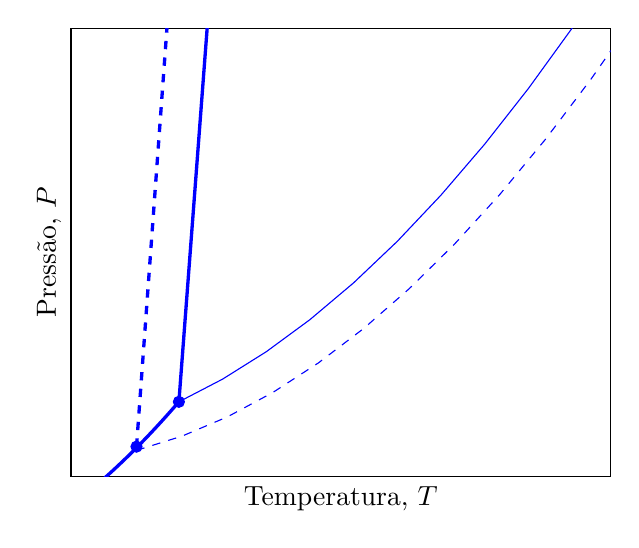
\begin{tikzpicture}
\begin{axis}
    [
        grid = major,
        ylabel = {Pressão, $P$},
        xlabel = {Temperatura, $T$},
        ymin=10, ymax=40,
        xmin=-70, xmax=0,
        ytick = \empty,
        xtick = \empty,
    ]       
    \draw [draw=blue, very thick]
        (axis cs: -100, 2) parabola 
        (axis cs: -56, 15);
    \addplot [blue, domain=-56:80]
        { x^2/204 + (161*x)/204 + 745/17 };
    \draw [draw=blue, very thick]
        (axis cs: -56, 15) -- 
        (axis cs: -45, 90);

    \addplot [blue, domain=-61.5:80, dashed]
        { (x-5.5)^2/204 + (161*(x-5.5))/204 + 745/17 - 1.2 };
    \draw [draw=blue, very thick, dashed]
        (axis cs: -61.5, 12) -- 
        (axis cs: -50.5, 90);
    
    \addplot [ mark=*, color=blue, only marks ] coordinates
        { 
            (-56, 15)
            (-61.5, 12)
        };
        
\end{axis}
\end{tikzpicture}
